\documentclass[10pt,twocolumn,letterpaper]{article}

\usepackage{cvpr}
\usepackage{times}
\usepackage{epsfig}
\usepackage{graphicx}
\usepackage{amsmath}
\usepackage{amssymb}
\usepackage{bbm}


% Include other packages here, before hyperref.

% If you comment hyperref and then uncomment it, you should delete
% egpaper.aux before re-running latex.  (Or just hit 'q' on the first latex
% run, let it finish, and you should be clear).
\usepackage[breaklinks=true,bookmarks=false]{hyperref}

\cvprfinalcopy % *** Uncomment this line for the final submission

\def\cvprPaperID{****} % *** Enter the CVPR Paper ID here
\def\httilde{\mbox{\tt\raisebox{-.5ex}{\symbol{126}}}}

% Pages are numbered in submission mode, and unnumbered in camera-ready
%\ifcvprfinal\pagestyle{empty}\fi
\begin{document}

%%%%%%%%% TITLE
\title{Twist to Grasp: Rotational Region Proposals for Grasp Detection}

\author{Chandler Watson\\
Stanford University\\
{\tt\small watsonc@stanford.edu}
% For a paper whose authors are all at the same institution,
% omit the following lines up until the closing ``}''.
% Additional authors and addresses can be added with ``\and'',
% just like the second author.
% To save space, use either the email address or home page, not both
\and
Michal Adamkiewicz\\
Stanford University\\
{\tt\small mikadam@stanford.edu}
}

\maketitle
%\thispagestyle{empty}

%%%%%%%%% ABSTRACT
\begin{abstract}
   The ability to autonomously grasp objects is a defining trait of humankind, and allows us to manipulate objects to better understand our environment; however, detecting where on an object to grasp is a difficult problem. The majority of current models for robotic grasp detection have focused on standard feed-forward convolutional neural networks, but a recently proposed model uses a Region Proposal Network (RPN) architecture to propose and refine grasps. To deal with the difficulty of regressing over the rotation parameter, $\theta$, this paper discretizes $\theta$ and uses a softmax layer to determine $\theta$'s value. Just one month later, a paper was released outlining a model for detecting arbitrarily-oriented text in an image with Rotation Region Proposal Networks (RRPNs). In this paper, we propose a synthesis of these two models, retaining the former model's softmax layer, but using its value $\Delta \theta$ to refine a rotation region proposal, improving the models initial predictions and minimizing the values which $\theta$ must range over. This model proved too difficult to implement in the time frame available, but we systematically motivate this model and characterize the dataset at hand, the Cornell grasping dataset, with a series of more readily constructible networks.
\end{abstract}

%%%%%%%%% BODY TEXT
\section{Introduction}

Teaching robots how to grasp objects is an intricate challenge with many components. Whereas humans can simply reach down and pick an object up, a robot must first recognize the object, find an intelligent location on the object to grasp it, plan and control the motion of its arm down to the object, and perform the intended grasp. Motion planning and control for robotic grasping can be handled by classical methods, such as~\cite{chitta12}, but grasp detection is somewhat difficult using classical methods, necessitating a deeper understanding of the physical shape of the object in question.

Although early approaches focused on compiling classical visual features, the current state of grasp detection lies entirely within the realm of convolutional neural networks. A model~\cite{redmon14} based on the Zeiler and Fergus architecture in 2014 set the stage for a vast series of later networks, growing deeper and deeper until the release of Deep Grasp~\cite{vela2018}. Deep Grasp is a grasp detection network built on a ResNet-50 backbone with a Region Proposal Network (RPN) in the middle. At the end of the ResNet-50, a single softmax layer selects a discretized value for $\theta$, the rotation parameter, and another fully connected layer refines the bounding box parameters as in Faster-RCNN~\cite{ren15}. Deep Grasp proceeded to achieve state of the art results on the Cornell grasping dataset with 96.0\% test accuracy.

Just one month after the publication of Deep Grasp, a second paper by Ma et al.~\cite{ma18} outlined a method for modifying the standard RPN into a rotation RPN, or RRPN. By choosing a discrete set of angles, ~\cite{ma18} defines a RPN with angled anchors, allowing for rotated proposals. These are scored as in Faster-RCNN~\cite{ren15} and region of interest (RoI) pooling is performed by pooling at the same angle as a given proposal. Standard smooth-$L_1$ loss is used for bounding box regression, and binary cross entropy loss is used for background classification. The architecture as a whole remains analogous to~\cite{ren15}. 

Because Deep Grasp's RPN yields bounding boxes without rotation, the latter part of the Deep Grasp network has to handle all of the rotational prediction within the last residual block of its ResNet backbone. Furthermore, a non-oriented bounding box could potentially constrain grasps to be either poorly oriented or too small for an appropriate grasp. This issue is most likely to arise in dense clutter, where bounding boxes may need to fit objects closer.

We propose an alternate network formulation based on RRPNs, allowing for more versatile bounding box predictions and thus more robust grasp prediction results. By allowing for orientation in both the RPN section of the network and in the final grasp prediction, we allow our model freedom to chose more appropriate bounding boxes and ultimately select better grasps. Furthermore, by relegating the final $\theta$ softmax layer to a refining role, we allow theoretically greater granularity for predicted angles. To our knowledge, no previous model has used any variant of RRPNs, and only Deep Grasp has made use of RPNs in general. 


\section{Related Work}


The earliest of models, including~\cite{edelman96}, used simple, hand-engineered features to detect grasp quality. Later, as neural networks rose in popularity, increasingly deep neural networks were applied to grasping ~\cite{pinto2015},~\cite{redmon14}. The most successful of these were convolutional neural networks, which steadily grew in size over time. ~\cite{redmon14}'s AlexNet-based architecture was able to achieve 88.0\% image-wise on the Cornell grasping dataset, which contains hundreds of RGB-D images of objects with potential grasps superimposed. A 5D grasp representation is given as in Figure $\ref{fig:grasp}$.

~\cite{kumra16} was able to achieve 90.0\% using a multi-modal architecture which passes the RGB and depth data through separate ResNet-50s, merging the resultant features and passing them through a three-layer fully-connected network. At about the same time,~\cite{guo17} managed to achieve 93.2\% image-wise accuracy with a simple feed-forward architecture based the ZF model, using L1 loss for bounding box prediction as inspired by Fast-RCNN. Of particular note is that a common design choice among these architectures is to discretize the angle parameter, and perform classification instead of regression, which appears to correlate with better performance.

\begin{figure}
    \centering
    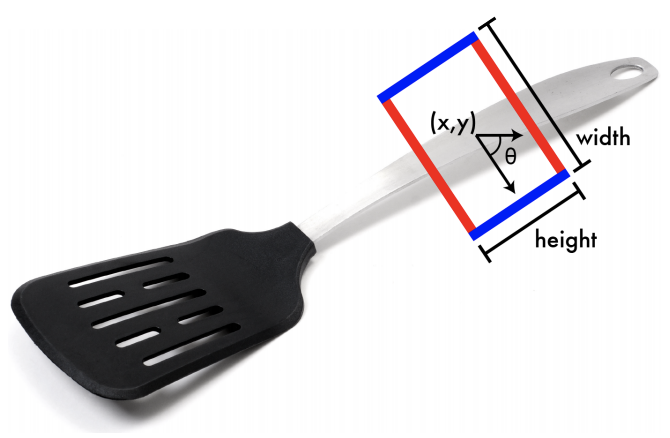
\includegraphics[width=0.4\textwidth]{latex/grasp.png}
    \caption{An example 5D grasp, from~\cite{redmon14}.}
    \label{fig:grasp}
\end{figure}

Today, the state of the art for the Cornell grasping dataset is DeepGrasp~\cite{vela2018}, a 100+ layer ResNet-based architecture including a region proposal network (RPN) allowing the network all the speed benefits of Faster R-CNN. A full RGB-D image is passed through the first three residual blocks of a ResNet-50 network for feature extraction, resulting in a feature map. The results from a grasp proposal network are then combined with these features and passed through a ROI pooling layer. The resultant values are then passed back into the ResNet-50 network, and then through fully-connected layers to perform discredited regression on the grasp rectangle coordinates and the angle. The whole network is depicted in Figure $\ref{fig:deepgrasp}$.

Just after the publication of~\cite{vela2018}, a second publication~\cite{ma18} proposed a region proposal network designed for rotated text detection. The model in question, Rotation Region Proposal Networks (RRPN), has a VGG-16 backbone, and is structured analogously to Faster-RCNN~\cite{ren15}. The anchors (and thus proposals) have an additional discrete angle parameter, as well as the typical ratio and scale parameters. Additionally, the IoU computation for proposal refinement and the ROI pooling layer are modified to allow for robust handling of rotated bounding boxes. See Figure \ref{fig:rrpn}.

\begin{figure}
    \centering
    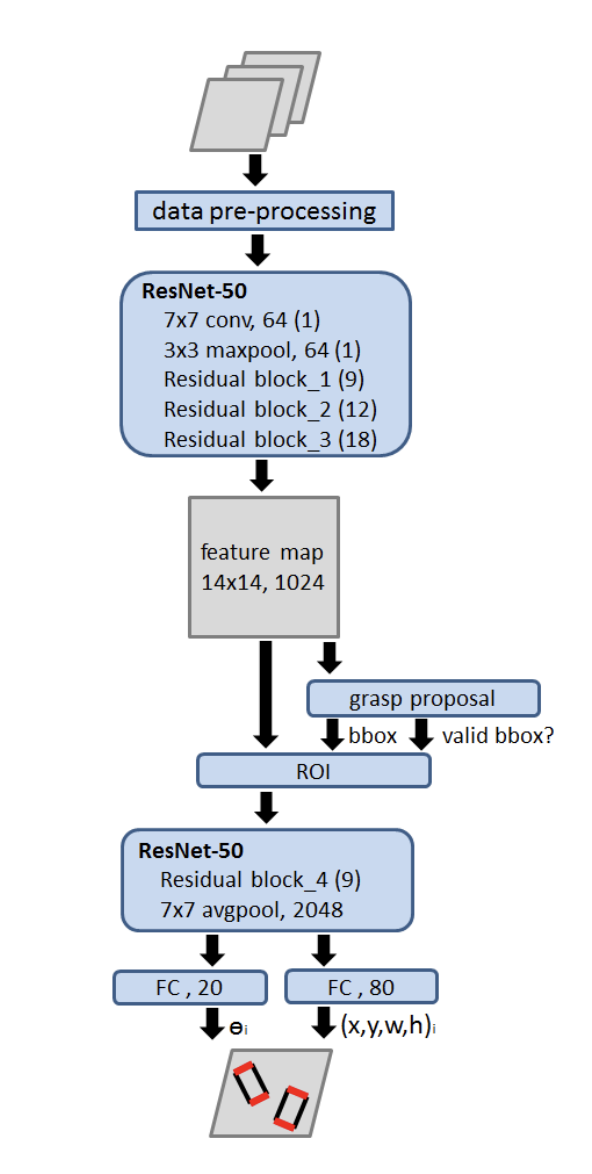
\includegraphics[width=0.25\textwidth]{latex/deepgrasp.png}
    \caption{The original DeepGrasp architecture, from~\cite{vela2018}.}
    \label{fig:deepgrasp}
\end{figure}




\section{Data}


The current standard data set for the 2D grasping task is the Cornell Grasping Data set \cite{cornelldataset}. It consists of 1035 images RGB-D images depicting 280 household objects on a white background. Each object is photographed from a variety of different angles over multiple images. The data set contains human annotated grasp rectangles, internally represented as sets of four points, for use during training.

Additionally, the dataset contains 11 background images of the backdrop without any graspable object, along with a map of which images correspond to which backgrounds. Due to the architectural nature of convolutional neural networks, these tend to go unused by most modern papers, and continue to go unused here.

In the majority of modern papers, following the pattern set by~\cite{redmon14}, grasps are represented by a 5-tuple as shown in Figure \ref{fig:grasp}. This is the pattern used by Deep Grasp, and in fact is used in the internal RPN, matching Faster-RCNN's $(x, y, w, h)$ proposals. 


\begin{figure}
    \centering
    
\begin{tabular}{cc}

	  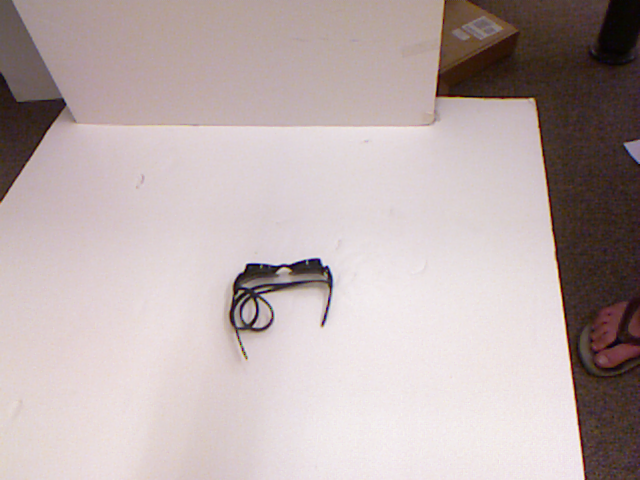
\includegraphics[width=0.22\textwidth]{images/googles.png} & 
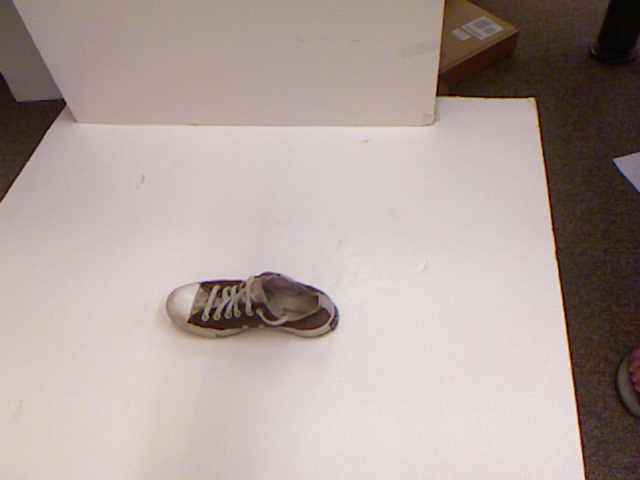
\includegraphics[width=0.22\textwidth]{images/shoe.png} \\

\end{tabular}

    \caption{Examples from the Cornell dataset~\cite{cornelldataset}.}
\end{figure}



Our model is designed to take in a single RGB-D image of a graspable object with corresponding depth map, and output a five-dimensional grasp as described in \cite{vela2018}:
$$g = \{x, y, \theta, w, h\}$$ 
where $(x, y)$ is the center of the bounding box, $\theta$ is the orientation, and $w$ and $h$ are the width and height (opening distance) of the gripper performing the grasp. Evaluation is performed as established in the literature by~\cite{redmon14} and used by DeepGrasp~\cite{vela2018}. For a grasp to be correct, it must be within $30^\circ$ of a ground truth grasp for the given object and the Jaccard index between the ground truth and the predicted grasp must be above $0.25$, where the Jaccard index is defined as
$$J(g_{pred}, g_{truth}) = \frac{|g_{pred} \cap g_{truth}|}{|g_{pred} \cup g_{truth}|}.$$
We test on both the original Cornell Dataset with 885 images of 244 distinct objects as in~\cite{redmon14} and~\cite{vela2018}. Additionally, we note for further testing that~\cite{vela2018} has provided their Multi-Object Dataset, containing which contains 96 images containing 3-5 objects per image. This dataset has not seen much use in the literature yet, but this is likely because~\cite{vela2018} was published just four months ago.

\begin{figure}
    \centering
    \hspace*{-0.8cm}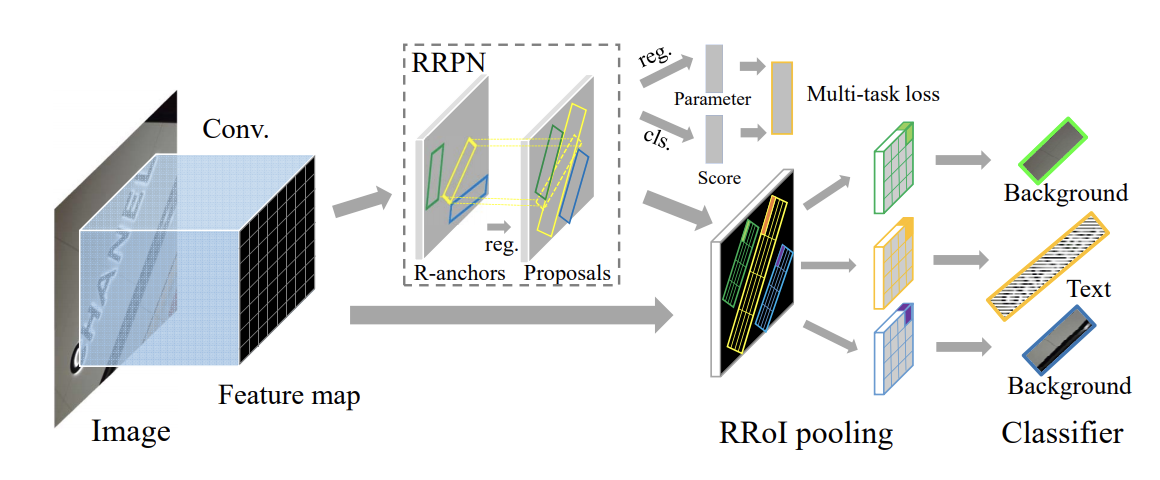
\includegraphics[width=0.55\textwidth]{latex/rrpn.png}
    \caption{The RRPN architecture, from~\cite{ma18}.}
    \label{fig:rrpn}
\end{figure}

\section{Methods}

We follow DeepGrasp~\cite{vela2018} in general architecture, as well as using ResNet-50 as a backbone. Preprocessed data is passed through the first part of ResNet-50 and through the first three residual blocks, then into a $14 \times 14 \times 1024$ feature map. These features are passed into a RRPN module, which predicts a bounding box and probability of the bounding box containing a valid grasp. Both of these as well as the feature map enter a Rotation Region-of-Interest (RRoI) pooling layer, which performs an analogue of standard RoI pooling on rotated regions of interest. Lastly, as in ~\cite{vela2018}, we pass the pooled features into the remainder of the ResNet-50, and use fully-connected layers to perform discretized regression on the grasp orientation (our $\Delta \theta$) and refine the grasp from our bounding box. Note that, at the end, the orientation is reported as the sum of the bounding box orientation and the predicted grasp orientation. 

The anchor strategy is similar to~\cite{ma18}, but uses smaller ratios (i.e. only 1:1 or 1:2). During experimentation, number of angles, ratios, etc. are treated as hyperparmeters. We propose that the number of angles for the anchors should divide the number of discretized grasp angles to allow a better possibility of the bounding box choosing the proper angle \textit{a priori}, and consider restricting the gripper orientation within the box to a smaller set of angles. A standard choice could thus be 

Data preprocessing is identical to that given in $\cite{vela2018}$. We follow $\cite{vela2018}$ in following $\cite{redmon14}$ in replacing the blue channel in the ResNet-50 backbone with the depth channel to reuse pretrained weights, adjusting it to a 0 to 255 range. Data augmentation is done by center-cropping to $351 \times 351$ images, followed by a random rotation and secondary crop to $321 \times 321$. A random translation from 0 to 50 pixels in both $x$ and $y$ follows, and the resulting image is resized to $224 \times 224$, acceptable to ResNet-50. Whereas data augmentation is performed ahead of time in $\cite{ma18}$, resulting in a set of 1,000 images, we perform data augmentation as part of a PyTorch Dataset pipeline, resulting in a continuous stream of unseen images at train time. 

Loss is calculated similarly to both~\cite{vela2018} and~\cite{ma18}, which use multi-task loss analogous to that of Faster-RCNN~\cite{ren15}. In particular, we use~\cite{vela2018}'s loss function, but replace the component grasp proposal network losses with their counterparts in~\cite{ma18}. In turn, we retain the softmax layer for $\theta$, but significantly reduce its range, making it an additive contribution to the region proposal. This maintains DeepGrasp's approach to regressing over $\theta$ while augmenting it by minimizing the range $\theta$ necessarily must range over. In full, our loss takes the form $L = L_{gpn} + L_{gcr}$ where
\begin{align}
    L_{gpn}(\{(p_i, t_i)_{i=1}^I\}) &= \sum_i L_{gpn\_cls}(p_i, p_i^*)\\
    &+ \lambda_1 \sum_i p_i^* L_{gpn\_reg}(t_i, t_i^*) \nonumber\\
    L_{gcr}(\{(\rho_l, \beta_l)\}_{c=0}^C) &= \sum_c L_{gcr\_cls}(\rho_l)\\
    &+ \lambda_2 \sum_c \mathbbm{1}_{c \neq 0}(c) L_{gcr\_reg}(\beta_c, \beta_c^*) \nonumber
\end{align}
\begin{align}
    L_{gpn\_cls}(p_i, p_i^*) &= -p_i^* \log p_i\\
    &- (1-p_i^*) \log (1-p_i) \nonumber\\
    L_{gpn\_reg}(t_i, t_i^*) &= \sum_{j} \text{smooth}_{L_1}((t_i^*)_j-(t_i)_j)
\end{align}

and $L_{gcr\_cls}$ and $L_{gcr\_reg}$ are calculated as usual (i.e. as in Faster-RCNN or, consequently, Deep Grasp), with multi-class cross entropy loss and smooth-L1 loss.

\section{Experiments}

We train Deep Grasp and our model, hereafter called Deep Twist, side by side on the Cornell dataset. The standard Deep Grasp preprocessing as described above is used for both. For comparison and to help characterize the dataset, we run three baseline models as well. These are networks with the same discretized $\theta$ and bounding box output as Deep Grasp and Deep Twist, but instead of using these as refinements to an existing bounding box, we use them as direct values. For feature extraction, we use ResNet-50, VGG16, and AlexNet. We train each feature extractor with smooth L1 and L2 bounding box loss to highlight the importance of using smooth L1 loss and shine light on issues we had training early baseline models. 

Due to the unexpected difficulty of constructing a model for Deep Grasp, the two primary models of this paper currently have no data. This is due in large part to the current difficulty of assembling RPN-based models while working with Autograd, especially with operations such as RoI pooling. As PyTorch is in development, it has been the case that a number of critical key functions don't have backwards passes written for them, causing a number of key PyTorch implementations (pytorch-faster-rcnn, simple-faster-rcnn-pytorch) of such models to resort to using CUDA kernels which conflicted with our setup. The one existing public implementation (faster-rcnn.pytorch) that claimed to have CPU support led to issues had a data loading process that was nearly impossible to decipher, as it was built off a series of other Faster-RCNN implementations carrying a data storage format which was rather convoluted and would have taken significantly more time to work with. We ultimately returned back to attempting to construct a Deep Grasp setup based on our framework, but this most importantly demonstrated the need for clear, well-documented RPN-based models in the PyTorch community. 

Despite these setbacks, we continue, presenting a characterization of the dataset by training the aforementioned baseline models on the Deep Grasp dataset, presenting visualizations of their training, and giving a brief theoretical justification for our model. The results are given in Figure \ref{fig:table} and discussed further here. 

\begin{figure}
    \label{fig:table}
    \begin{center}
        \begin{tabular}{c|cc}
            \hline
            Model: & Test Accuracy (Epoch 10)\\
            \hline
            Resnet-50, Smooth L1 & 23.16\% \\
            \hline
            ResNet-50, L2 & 15.82\% \\
            \hline
            VGG16, Smooth L1 & 0.00\% \\
            \hline
            VGG16, L2 & 0.00\% \\
            \hline
            AlexNet, Smooth L1 & 0.00\% \\
            \hline
            AlexNet, L2 & 15.25\% \\
            \hline
            
        \end{tabular}
    \end{center}
    \caption{Early test accuracies for various architectures.}
\end{figure}

We note that by recording early test accuracies, some of the baseline models perform very well (up to $23.16\%$) for just 10 epochs, whereas others appear not to perform well at all. Of particular note is the AlexNet smooth L1 model, which appears to find a relatively low-cost local minimum, yet has zero accuracy on both the training and test sets. The loss appears to waver from example to example (as expected, especially given the random aspect of the prepossessing) yet always seems to hover about the same value. 

The VGG16 network with L2 loss exhibited similar behavior, but the loss would oscillate in the range of $10^{16}$ despite using Kaiming initialization. The last VGG16 network had been stopped prematurely, and very well could have converged nicely as well.

\begin{figure}
    \centering
    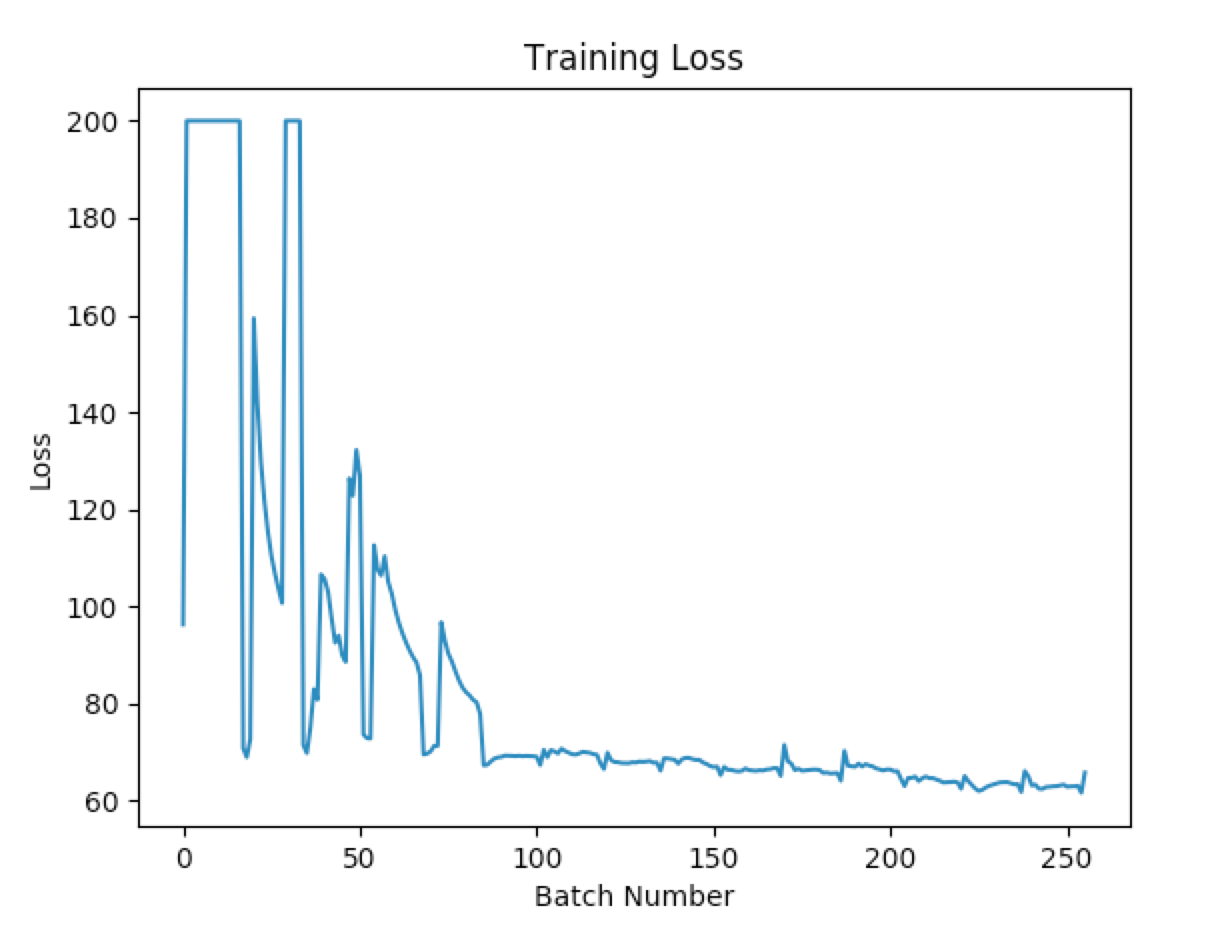
\includegraphics[width=0.5\textwidth]{images/lossovertime.png}
    \caption{Loss over time of AlexNet with smooth L1 loss, achieving zero accuracy}
\end{figure}


\begin{figure}
    \centering
    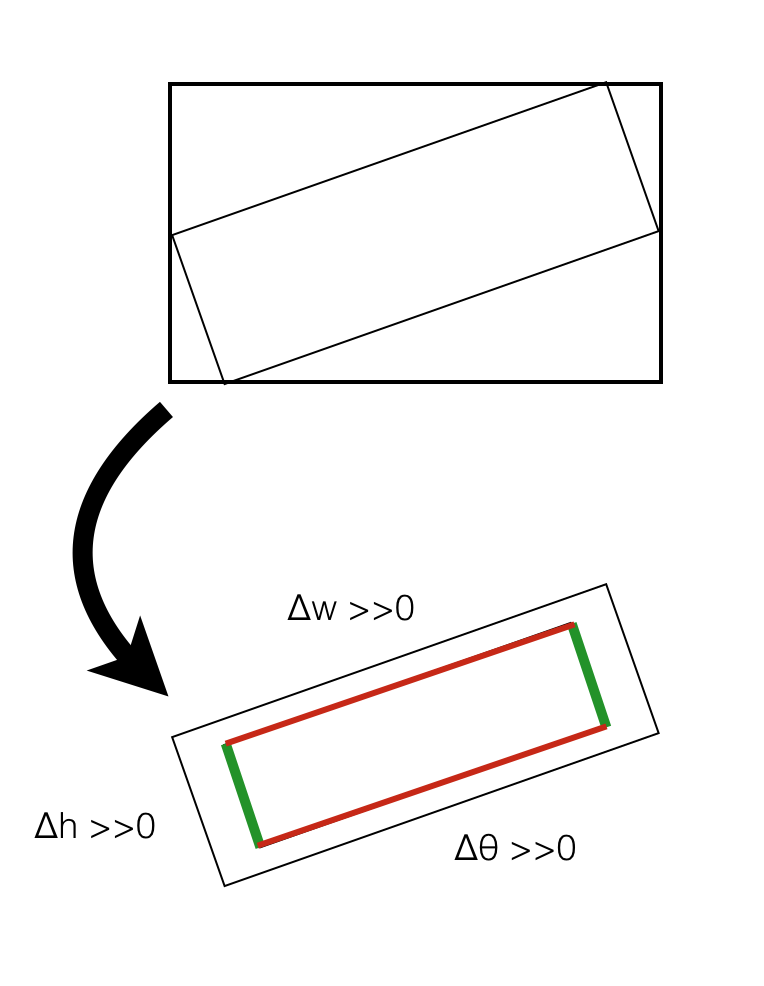
\includegraphics[width=0.5\textwidth]{images/diagram.png}
    \caption{Diagram demonstrating a deficiency of Deep Grasp. Deep Grasp must use a large bounding box to view the edges of the gripper, then use a single residual block to shrink the bounding box to the right size. We hypothesize this would become a very significant issue in dense clutter.}
\end{figure}


\subsection*{Visualization of Training}

While training, we noted that the AlexNet model with smooth L1 loss had somehow found a local minimum that consistently yielded zero accuracy on training examples it was given. At the start of training, loss appears to spike, then reduces quickly and settles at this same minimum. From further visual inspection, the disappearance of predicted grasps from the image suggests that relative scaling of loss terms appears to be the issue, not anything intrinsic to the problem itself. Indeed, simple models seem to be able to train rather quickly, and given sufficient compute, it seems as though a ResNet-50 based simple feed-forward model could quickly compare with $\cite{redmon14}$'s accuracy while maintaining faster evaluation speed than Deep Grasp. 

\begin{figure}
    \label{fig:example}
    \centering
    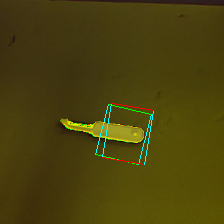
\includegraphics{latex/whoa-3-199.png}
    \caption{An example diagnostic grasp prediction from a ResNet-50 model, demonstrating intentional overfitting.}
    \label{fig:my_label}
\end{figure}


\subsection*{Theoretical Reasoning}

We now give an informal argument for the advantages of Deep Twist over Deep Grasp. We trivially note that for any predicted grasp $t_i$, it is possible that Deep Twist's RRPN proposal can match the box exactly, simply by matching the parameters of the existing box. This, however, is not true for Deep Grasp, as any rotation will yield either area missed or area not covered. The choice of region that puts the least responsibility on the last residual block of the network is having the region be exactly an angle-reset version of the ground truth grasp. However, such an assignment clearly misses the edges of the grasp, the most crucial part to determining not only orientation but grasp confidence scores as well. Therefore, Deep Grasp is forced to fit a region around the entire network, which can include many spurious features if the rectangle is at a skew angle. Additionally, the latter part of the network is then forced to take the existing bounding box and communicate via only convolutional features the difference in each length parameter necessary. The immediately obvious fix would be if the original bounding box could capture the edges of the grasp region while remaining close in parameter space to the grasp itself. The design of Deep Twist does this exactly.

Another benefit of Deep Twist over previous approaches is that it should scale better to higher dimensional problems. In the case of 2.5D grasping one merely has to worry about one angle; performing classification over it results in only $20$ possible configurations. However, in the case of a 3D grasping problem, one requires 3 Euler angles, which to achieve a similar accuracy necessitates $20^3 = 8000$ softmax units. By minimizing the range of $\theta$, we allow far greater granularity and require fewer discrete values of $\theta$.

\subsection*{Future Directions}

In lieu of finishing the construction of the Deep Twist model, we give a number of illustrative paths for future research. In addition to the creation of well-documented, easy to use RPN-based models, we suggest that future exploration work toward the use of innovative representations for region proposals. For instance, one clever representation of 3D rotations is the Lie group $SE(3)$, which seems to be somewhat popular in robotics research \cite{liegroups} and allows for simple representation of rotations without having to worry about parameter bounds. We therefore suggest that an extension of~\cite{ma18} to 3D cases could utilize such a parametrization. 

The unique nature of Deep Twist allows us to easily generalize the model to higher dimensions. This is due to primarily relying on regression over the angle as opposed to classification, opening the possibility of more for more general environmental manipulation tasks. In combination with a clever representation, this could allow for a far more robust solution to 3D pose representation than a massive softmax layer, building angular similarity into the representation rather than requiring it to be learned in several repetitive convolutional features.

Along this vein is the use of rotational invariant convolution as proposed in \cite{RotationInvariance} and \cite{RotationInvarianceVHS}. In the same way convolutions neural network layers are invariant to translation the proposed model are invariant to rotations on the input images. We think this would yield itself very well to the grasping application as there isn't a preferred down direction for the images to be taken in. This would allow us to generalize better to unseen orientations of objects.

\section{Conclusion}

In this paper, we have given an in-depth discussion of RPN-based grasp detection networks, proposed Deep Twist, a convolutional network designed to improve upon Deep Grasp~\cite{vela2018} by utilizing Rotational RPNs~\cite{ma18}, and performed preliminary experimentation with the Cornell dataset to demonstrate the efficiacy of the convolutional paradigm in this relatively obscure computer vision problem. Lastly, we have proposed a series of possible continuations regarding the use and implementation of Deep Twist in 3D environments, allowing for more advanced robotic manipulation.

{\small
\bibliographystyle{ieee}
\bibliography{egbib}
}

\end{document}
